\chapter{2023/12/11}\label{20231211}

\emph{场论由 Faraday 于 1865
年提出,第一次运用是在笔记中出现了``field''这个词}

\emph{7岁学习微积分的陶哲轩大神:``直觉'' (intuition)}

\section{Two paradigms for classical mechanics
经典力学的两大范式}\label{two-paradigms-for-classical-mechanics-ux7ecfux5178ux529bux5b66ux7684ux4e24ux5927ux8303ux5f0f}

\textbf{Paradigm I:} Newton's 1st principle (第一性原理)

\textbf{Paradigm II:} Kepler's big data (大数据)

Kepler's big data established paradigms for all subjects.

\section{Data-driven (re)discovery of partial differential equations
数据驱动下对偏微分方程的(重)发现}\label{data-driven-rediscovery-of-partial-differential-equations-ux6570ux636eux9a71ux52a8ux4e0bux5bf9ux504fux5faeux5206ux65b9ux7a0bux7684ux91cdux53d1ux73b0}

From \emph{Science Advances}, \emph{Data-driven discovery of partial differential equations} (\url{https://doi.org/10.1126/sciadv.1602614}).

Examples:
\begin{itemize}
    \tightlist{}
    \item Navier-Stokes equations 纳维-斯托克斯方程 \[ {\partial \boldsymbol v \over \partial t} +(\boldsymbol v \cdot \nabla) \boldsymbol v = - {1 \over \rho} \nabla p + \mu \nabla^2 \boldsymbol v + \boldsymbol g\]
    \item Schrödinger Equation 薛定谔方程
    \[-{ \hbar^2 \over 2m } \nabla ^2 \psi + U \psi =i\hbar {\partial \psi \over \partial t}\]
    \item Korteweg--De Vries equation 科特韦赫-德弗里斯方程 / KdV方程
    \[\partial_t \phi + \partial^3_x \phi - 6 \phi \partial_x \phi =0\]
\end{itemize}

\section{Four paradigms
四种范式}\label{four-paradigms-ux56dbux79cdux8303ux5f0f}

For future reference, you can see the book
\emph{The Fourth Paradigm: Data-intensive Scientific Discovery} (2009) (\url{https://www.microsoft.com/en-us/research/uploads/prod/2009/10/Fourth_Paradigm.pdf}).

\begin{center}
    \begin{tabular}{|c|c|c|}
        \hline
        \textbf{Order} & \textbf{Contents} & \textbf{Base} \\
        \hline
        1st Paradigm & Experimental-based empirical science & Experiments \\
        \hline
        2nd Paradigm & Model-based theoretical science & Theoretical derivation \\
        \hline
        3rd Paradigm & Simulation-based numerical science & Computer simulations \\
        \hline
        4th Paradigm & Data-driven AI science & AI \\
        \hline
    \end{tabular}
    \captionof{table}{Four Paradigms in Science}
\end{center}

\begin{quote}
思考:第三点和第四点有什么区别?
\end{quote}

\section{AI for science
汤超院士:AI的三个层次}\label{ai-for-science-ux6c64ux8d85ux9662ux58ebaiux7684ux4e09ux4e2aux5c42ux6b21}

For the full text of Tang Chao's speech, please turn to the webpage \emph{2022科学智能峰会回顾|汤超院士:关于AI for Science的几层意思} (\url{http://www.aais.pku.edu.cn/news/shownews.php?id=1493}) for reference.

\emph{译者注:此部分先放中文在放英文,是因为原文为中文}

Tang Chao pointed out that there are 3 levels of AI application
nowadays:

\begin{enumerate}
\def\labelenumi{\arabic{enumi}.}
\item
  将深度学习技术用于各个学科中的科研、技术创新、成果转化等

  Applying deep learning technology to scientific research,
  technological innovation, and achievement transformation in various
  disciplines
\item
  利用AI来发现``new science''

  Using AI to discover ``new science''
\item
  AI背后的科学原理

  Science of AI
\end{enumerate}

Articles like \emph{Rediscovering orbital mechanics with machine learning} (\url{https://doi.org/10.1088/2632-2153/acfa63}) have pointed out that machine learning can be used to analyze big data and rediscover theorems in classical mechanics.

Researchers in the classical mechanics field should pay attention to
such advancements in AI and not stay away from them.

\section{Physical pendulum
物理摆}\label{physical-pendulum-ux7269ux7406ux6446}

\subsection*{(1) Random-shaped physical pendulum
一般的摆}\label{random-shaped-physical-pendulum-ux4e00ux822cux7684ux6446}

\begin{center}
    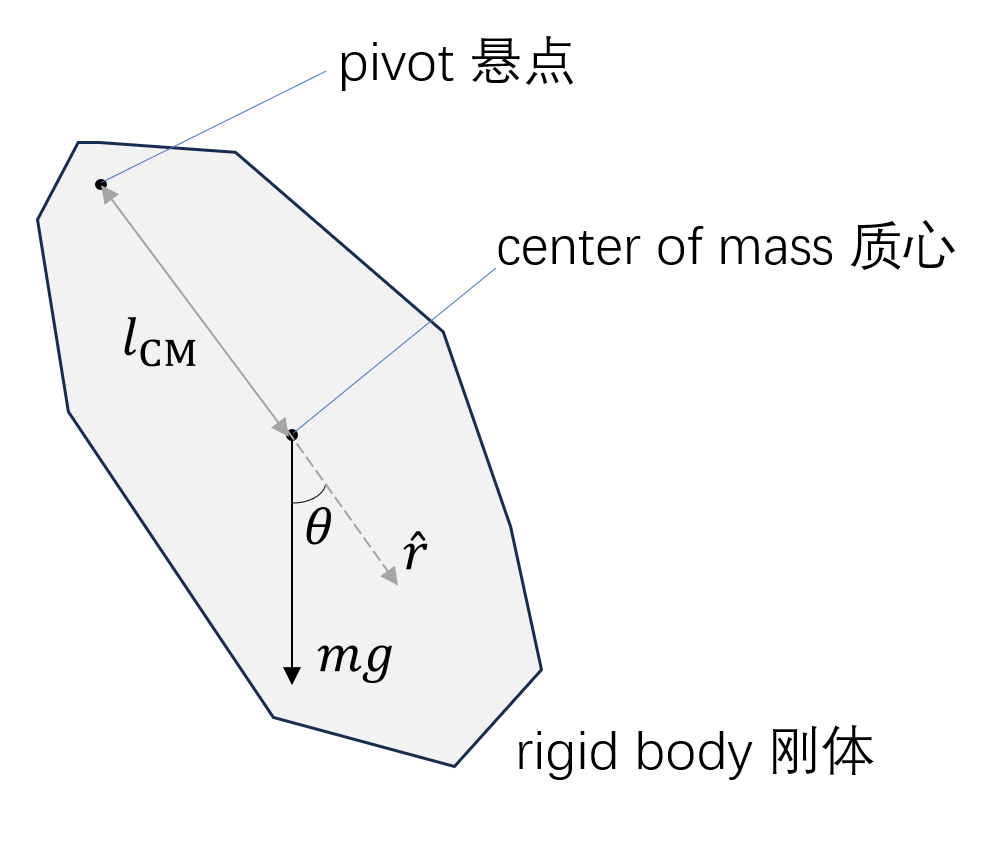
\includegraphics[height=150pt]{assets/Physical_pendulum.png}
    \captionof{figure}{Physical pendulum}
\end{center}

The gravity of the pendulum is
\[m\boldsymbol{g} = mg (\cos \theta \hat{\boldsymbol{r}} - \sin \theta \hat{\boldsymbol{\theta}}).\]

The torque is \begin{align*}
    \boldsymbol{M} & = \boldsymbol{r} \times m \boldsymbol{g} \\
    & = l_{\text{CM}} \hat{\boldsymbol{r}} \times mg (\cos \theta \hat{\boldsymbol{r}} - \sin \theta \hat{\boldsymbol{\theta}}) \\
    & = - l_{\text{CM}} mg \sin \theta \hat{\boldsymbol{k}}.
\end{align*}

According to the angular momentum theorem, we have
\[\boldsymbol{M} = - l_{\text{CM}} mg \sin \theta \hat{\boldsymbol{k}} = I \frac{\mathrm{d}^2 \theta}{\mathrm{d}t^2} \hat{\boldsymbol{k}}\]
\[I \ddot{\theta} + mgl_{\text{CM}} \sin \theta = 0.\]

When \(\theta \ll 1\),
\[\ddot{\theta} + \frac{mgl_{\text{CM}}}{I} \theta = 0.\]

\subsection*{(2) Torsional pendulum
扭摆}\label{torsional-pendulum-ux626dux6446}

\emph{编者吐槽:这图不会画}

Let the equilibrium position be \(\theta = 0\), and we know the torque
\[M = - k \theta.\]

Also, according to the angular momentum theorem,
\(M = I \ddot{\theta}\), and we have \[I \ddot{\theta} + k \theta = 0\]
\[\ddot{\theta} + \frac{k}{I} \theta = 0.\]

\section{Principle of virtual work/displacement
虚功/位移原理}\label{principle-of-virtual-workdisplacement-ux865aux529fux4f4dux79fbux539fux7406}

In a system with \(s\) degrees of freedom, we can write the position of
a particle \[\boldsymbol{r} = \boldsymbol{r}(q_1, q_2, \dots, q_s; t).\]

Take the time derivative of \(\boldsymbol{r}\) and we get
\[\boldsymbol{v} = \frac{\mathrm{d} \boldsymbol{r}}{\mathrm{d}t} = \frac{\partial \boldsymbol{r}}{\partial t} + \sum_{j = 1}^{s} \frac{\partial \boldsymbol{r}}{\partial q_j} \frac{\mathrm{d} q_j}{\mathrm{d}t}.\]

For a mechanical system at equilibrium, we know that
\[\delta W = \sum_{i = 1}^{n} \boldsymbol{F}_i \cdot \delta \boldsymbol{r}_i = \sum_{i = 1}^{n} \boldsymbol{F}_i \cdot \left( \sum_{j = 1}^{s} \frac{\partial \boldsymbol{r}_i}{\partial q_j} \delta q_j \right) = 0,\]
where \(n\) is the number of external forces applied on the system.

For each degree of freedom, there is a corresponding generalized force
\[Q_j = \sum_{i = 1}^{n} \boldsymbol{F}_i \cdot \frac{\partial \boldsymbol{r}_i}{\partial q_j}.\]

Also, we know that there are two types of forces: \textbf{active forces
(主动力)} and \textbf{constraint forces (约束力)}:
\[\boldsymbol{F}_i = \boldsymbol{F}_i^{\text{(a)}} + \boldsymbol{F}_i^{\text{(c)}},\]
and we can break \(\delta W\) into 2 parts:
\[\delta W = \sum_{i = 1}^{n} \sum_{j = 1}^{s} \boldsymbol{F}_i^{\text{(a)}} \cdot \frac{\partial \boldsymbol{r}_i}{\partial q_j} \delta q_j + \underline{\sum_{i = 1}^{n} \sum_{j = 1}^{s} \boldsymbol{F}_i^{\text{(c)}} \cdot \frac{\partial \boldsymbol{r}_i}{\partial q_j} \delta q_j}.\]

The underlined part (the work of the constraint forces) is usually
\(0\), and we only need to calculate the first part. That is,
\[\sum_{i = 1}^{n} \sum_{j = 1}^{n} \boldsymbol{F}_i^{\text{(a)}} \cdot \frac{\partial \boldsymbol{r}_i}{\partial q_j} \delta q_j = 0.\]
